\documentclass[11pt]{article}
\usepackage[margin=1in]{geometry}
\usepackage[T1]{fontenc}
\usepackage{lmodern,amsmath,amssymb,booktabs,graphicx,xcolor,hyperref}
\usepackage[numbers,sort&compress]{natbib}
\usepackage{tikz}
\usepackage{needspace,float}
\usetikzlibrary{arrows.meta,positioning}
\hypersetup{colorlinks=true,linkcolor=blue,citecolor=blue,urlcolor=blue}
\setlength{\emergencystretch}{2em}
\newcommand{\pending}[1]{\par\smallskip\Needspace{4\baselineskip}\noindent\textcolor{red!65!black}{\textbf{Draft completion item:} #1}\par\smallskip}
\newcommand{\kj}{\ensuremath{\mathrm{kJ\,mol^{-1}}}}
\renewcommand{\thefigure}{S\arabic{figure}}
\renewcommand{\thetable}{S\arabic{table}}
\title{Supporting Information: Route-Aware Computational Selection of Redox Motifs for Preformed Polymers}
\author{Working draft: authorship and affiliations to be confirmed}
\date{Evidence revision: 22 October 2026}
\begin{document}\maketitle
\noindent\textbf{Internal working draft.} This SI contains finite method controls and implementation checks. Pending scientific analyses remain explicit.
\section{Benchmark intervals and post hoc reference diagnostics}
The complete panel has 39 endpoints from 30 molecules and seven studies. Molecule-cluster 95\% percentile bootstrap intervals are [0.213,0.286] V for MAE, [0.245,0.313] V for RMSE and [0.128,0.257] V for bias. Study-cluster intervals are [0.178,0.306], [0.211,0.325] and [0.053,0.285] V, respectively. Both use 2,000 replicates and seed 20261021. The seven study clusters have unequal sizes; their percentile intervals are weakly calibrated. Molecule resampling retains common study and family effects and is also not a prediction interval for a new molecule.

For each cross-validation fold, a constant residual offset is estimated only from training endpoints and subtracted from the held-out prediction. Molecule and study folds remove all endpoints of the held-out molecule or DOI. The two-offset model fits separate constants for first and second redox steps. These choices were motivated by inspection of the complete retrospective panel and are internal diagnostics, not an untouched external test.
\begin{table}[htbp]\centering
\caption{Potential errors (V); primary unfitted statistics and internal offset diagnostics.}
\begin{tabular}{llrr}\toprule
Holdout & Offset model & MAE & RMSE\\\midrule
None & Unfitted, primary &0.247&0.279\\
Endpoint & One constant &0.157&0.210\\
Molecule & One constant &0.158&0.211\\
Study & One constant &0.182&0.232\\
Endpoint & Separate step constants &0.106&0.166\\
Molecule & Separate step constants &0.106&0.166\\
Study & Separate step constants &0.124&0.177\\\bottomrule
\end{tabular}\end{table}
Relative potentials to TEMPO, N-ethylphenothiazine, N-methylphthalimide and 1,4-benzoquinone cancel the computed ferrocene term algebraically. Each diagnostic excludes every endpoint of its anchor molecule. The resulting error includes the organic anchor's own model and measurement errors. Agreement after reference cancellation therefore does not uniquely identify a ferrocene error.
\begin{table}[htbp]\centering
\caption{Fc-independent relative-potential diagnostics; all endpoints of each organic anchor are excluded. Errors include the anchor's own model and experimental uncertainty.}
\begin{tabular}{lrrr}\toprule
Organic anchor & Endpoints & MAE (V) & RMSE (V)\\\midrule
TEMPO & 38 & 0.152 & 0.217\\
N-Ethylphenothiazine & 38 & 0.152 & 0.219\\
N-Methylphthalimide & 38 & 0.155 & 0.208\\
1,4-Benzoquinone & 37 & 0.168 & 0.250\\\bottomrule
\end{tabular}\end{table}


The spin-only partition includes multiplicity but omits an additional ferrocenium orbital contribution. Matrix spectroscopy and multireference calculations support a degenerate electronic ground state.\cite{fcorbital2017} An idealized additional twofold factor at 298.15 K would lower ferrocenium $G$ by 0.0178 eV, lower the computed Fc absolute potential by 0.0178 V and increase target potentials versus Fc by 0.0178 V. This limiting calculation would worsen the positive first-step bias. It is not an applied correction: solvent, orbital, vibronic and Jahn--Teller splittings are unresolved.
\section{Neutral-partner diffuse-basis sensitivity}
Five existing benchmark neutral partners were reoptimized with r$^2$SCAN, D4, def2-SVPD and SMD MeCN, with the same active $\omega$B97M-V/def2-TZVPD electronic-energy protocol and a separately checked SVPD Hessian. Each passed stationarity, spin, finite/symmetry, two-column/two-step derivative and minimum checks. A basis-independent certified qRRHO integrator and an independent partition reconstruction were used. No primary state, protocol label or certificate was replaced. Table~\ref{tab:basis} separates the change in nuclear thermal contribution from the active-energy change due to reoptimization. The existing reduced state and Fc reference are held fixed; only the neutral-partner contribution to the first potential is tested. These are combined reoptimization/Hessian sensitivities; thermal changes are not isolated fixed-geometry basis effects, and conformational relaxation can contribute.
\begin{table}[htbp]\centering
\caption{SVPD minus primary neutral-partner contributions, in meV; the total also equals the first-potential shift in mV.}
\label{tab:basis}
\begin{tabular}{lrrr}\toprule
Neutral partner & Nuclear & Geometry/SP & Total\\\midrule
1,4-Benzoquinone & -11.29 & -0.39 & -11.67\\
1,2-Naphthoquinone & -13.06 & -2.23 & -15.29\\
9,10-Phenanthrenequinone & -7.78 & -5.66 & -13.44\\
N-Methylphthalimide & -8.63 & -5.19 & -13.82\\
N,N'-Diisopropyl-PMDI & -21.27 & -13.81 & -35.08\\\bottomrule
\end{tabular}\end{table}
\section{Exact selected cases: partial assessment with explicit holds}
PMDI-ethyl and NDI-ethyl match enumerated exact designs by precursor, product and mapped new bond. All six redox states and the Fc reference were independently reconstructed; their existing grafting evidence hashes are unchanged. The registry now contains exact assessments rather than inherited family passes. Both remain held because the precise mono-N-ethyl/NH precursor access, attachment selectivity and experimental redox retention are unverified. The imide source establishes only a phthalimide/soluble-polymer analogue. Proposed DBU/MeCN conditions define the computed cycle and do not constitute a demonstrated synthesis protocol.
\begin{table}[htbp]\centering
\caption{Joined exact-case evidence. Potentials are V versus computed Fc; grafting free energies are \kj. Occupancy free energies remain uncomputed for these exact motifs.}
\begin{tabular}{lrrrrl}\toprule
Case & $E_1$ & $E_2$ & HCl route & DBU ions & Decision\\\midrule
PMDI-ethyl & -1.076 & -1.977 & -0.29 & -103.07 & Hold\\
NDI-ethyl & -0.764 & -1.418 & +10.05 & -92.73 & Hold\\\bottomrule
\end{tabular}\end{table}
Favorable model thermodynamics therefore do not override the route gate. These records identify the missing evidence and avoid duplicate full-redox jobs, but do not yet demonstrate a complete enumeration-to-occupancy selection.
\section{Relative-basicity controls}
The balanced reactions $\mathrm{B+DBUH^+\rightarrow BH^++DBU}$ avoid HCl, chloride and a free-proton reference. The exact pyridine, triethylamine and DBU identities match the revised author-maintained MeCN scale, with conjugate-acid pKa values 12.53, 18.83 and 24.31.\cite{basicity2019,pkaTables} Four new components and the two reused DBU components pass the same thermodynamic checks and an independent six-partition reconstruction. At 298.15 K, computed values are 71.82 and 32.68 \kj, compared with pKa-derived values 67.24 and 31.28 \kj; differences are $+4.58$ and $+1.40$ \kj. These values use the exact SI eV-to-molar-energy factor. Historical source records use 96.485 \kj/eV and are retained without replacement. Source temperature/activity qualifications remain open. This two-reaction control does not validate DIPEA, contact pairs or the complete grafting reaction and cannot assign the DBU/HCl discrepancy to a unique species. The separated model uses bare chloride in a continuum. Recent MeCN ion-solvation comparisons identify both species-dependent errors and sensitivity to absolute single-ion conventions, so the capture discrepancy cannot be assigned to chloride alone.\cite{pliego2024} Acid--chloride homoconjugation, such as $\mathrm{HCl+Cl^-\rightleftharpoons HCl_2^-}$, would introduce an additional species and acid-dependent speciation. It is not included in either ionic representation; no population or homoconjugation constant is inferred from the free-ion pKa comparison.
\section{Finite-polymer method controls}
Twenty-six of the original twenty-seven electronic oligomer cases currently pass geometry and active-energy checks. The open PMDI trimer has recovered and passed independent force checks. The stacked-start PMDI trimer returned optimizer convergence and saved active energies, but a later GPU-library call terminated abnormally. Separate final-force checks disagree with finite energy differences and remain unresolved, including a subsequent finer-step diagnostic. This case stays outside completed comparisons; no minimum or free energy is inferred from optimizer convergence alone. Construction and XYZ audits verify the intended open-chain topology. A trimer contains six backbone carbons, five backbone C--C bonds and two chain ends, rather than a triangular or cyclic backbone (Figure~\ref{fig:construction}). Proximity of pendant rings does not change that covalent connectivity.

\begin{figure}[htbp]
\centering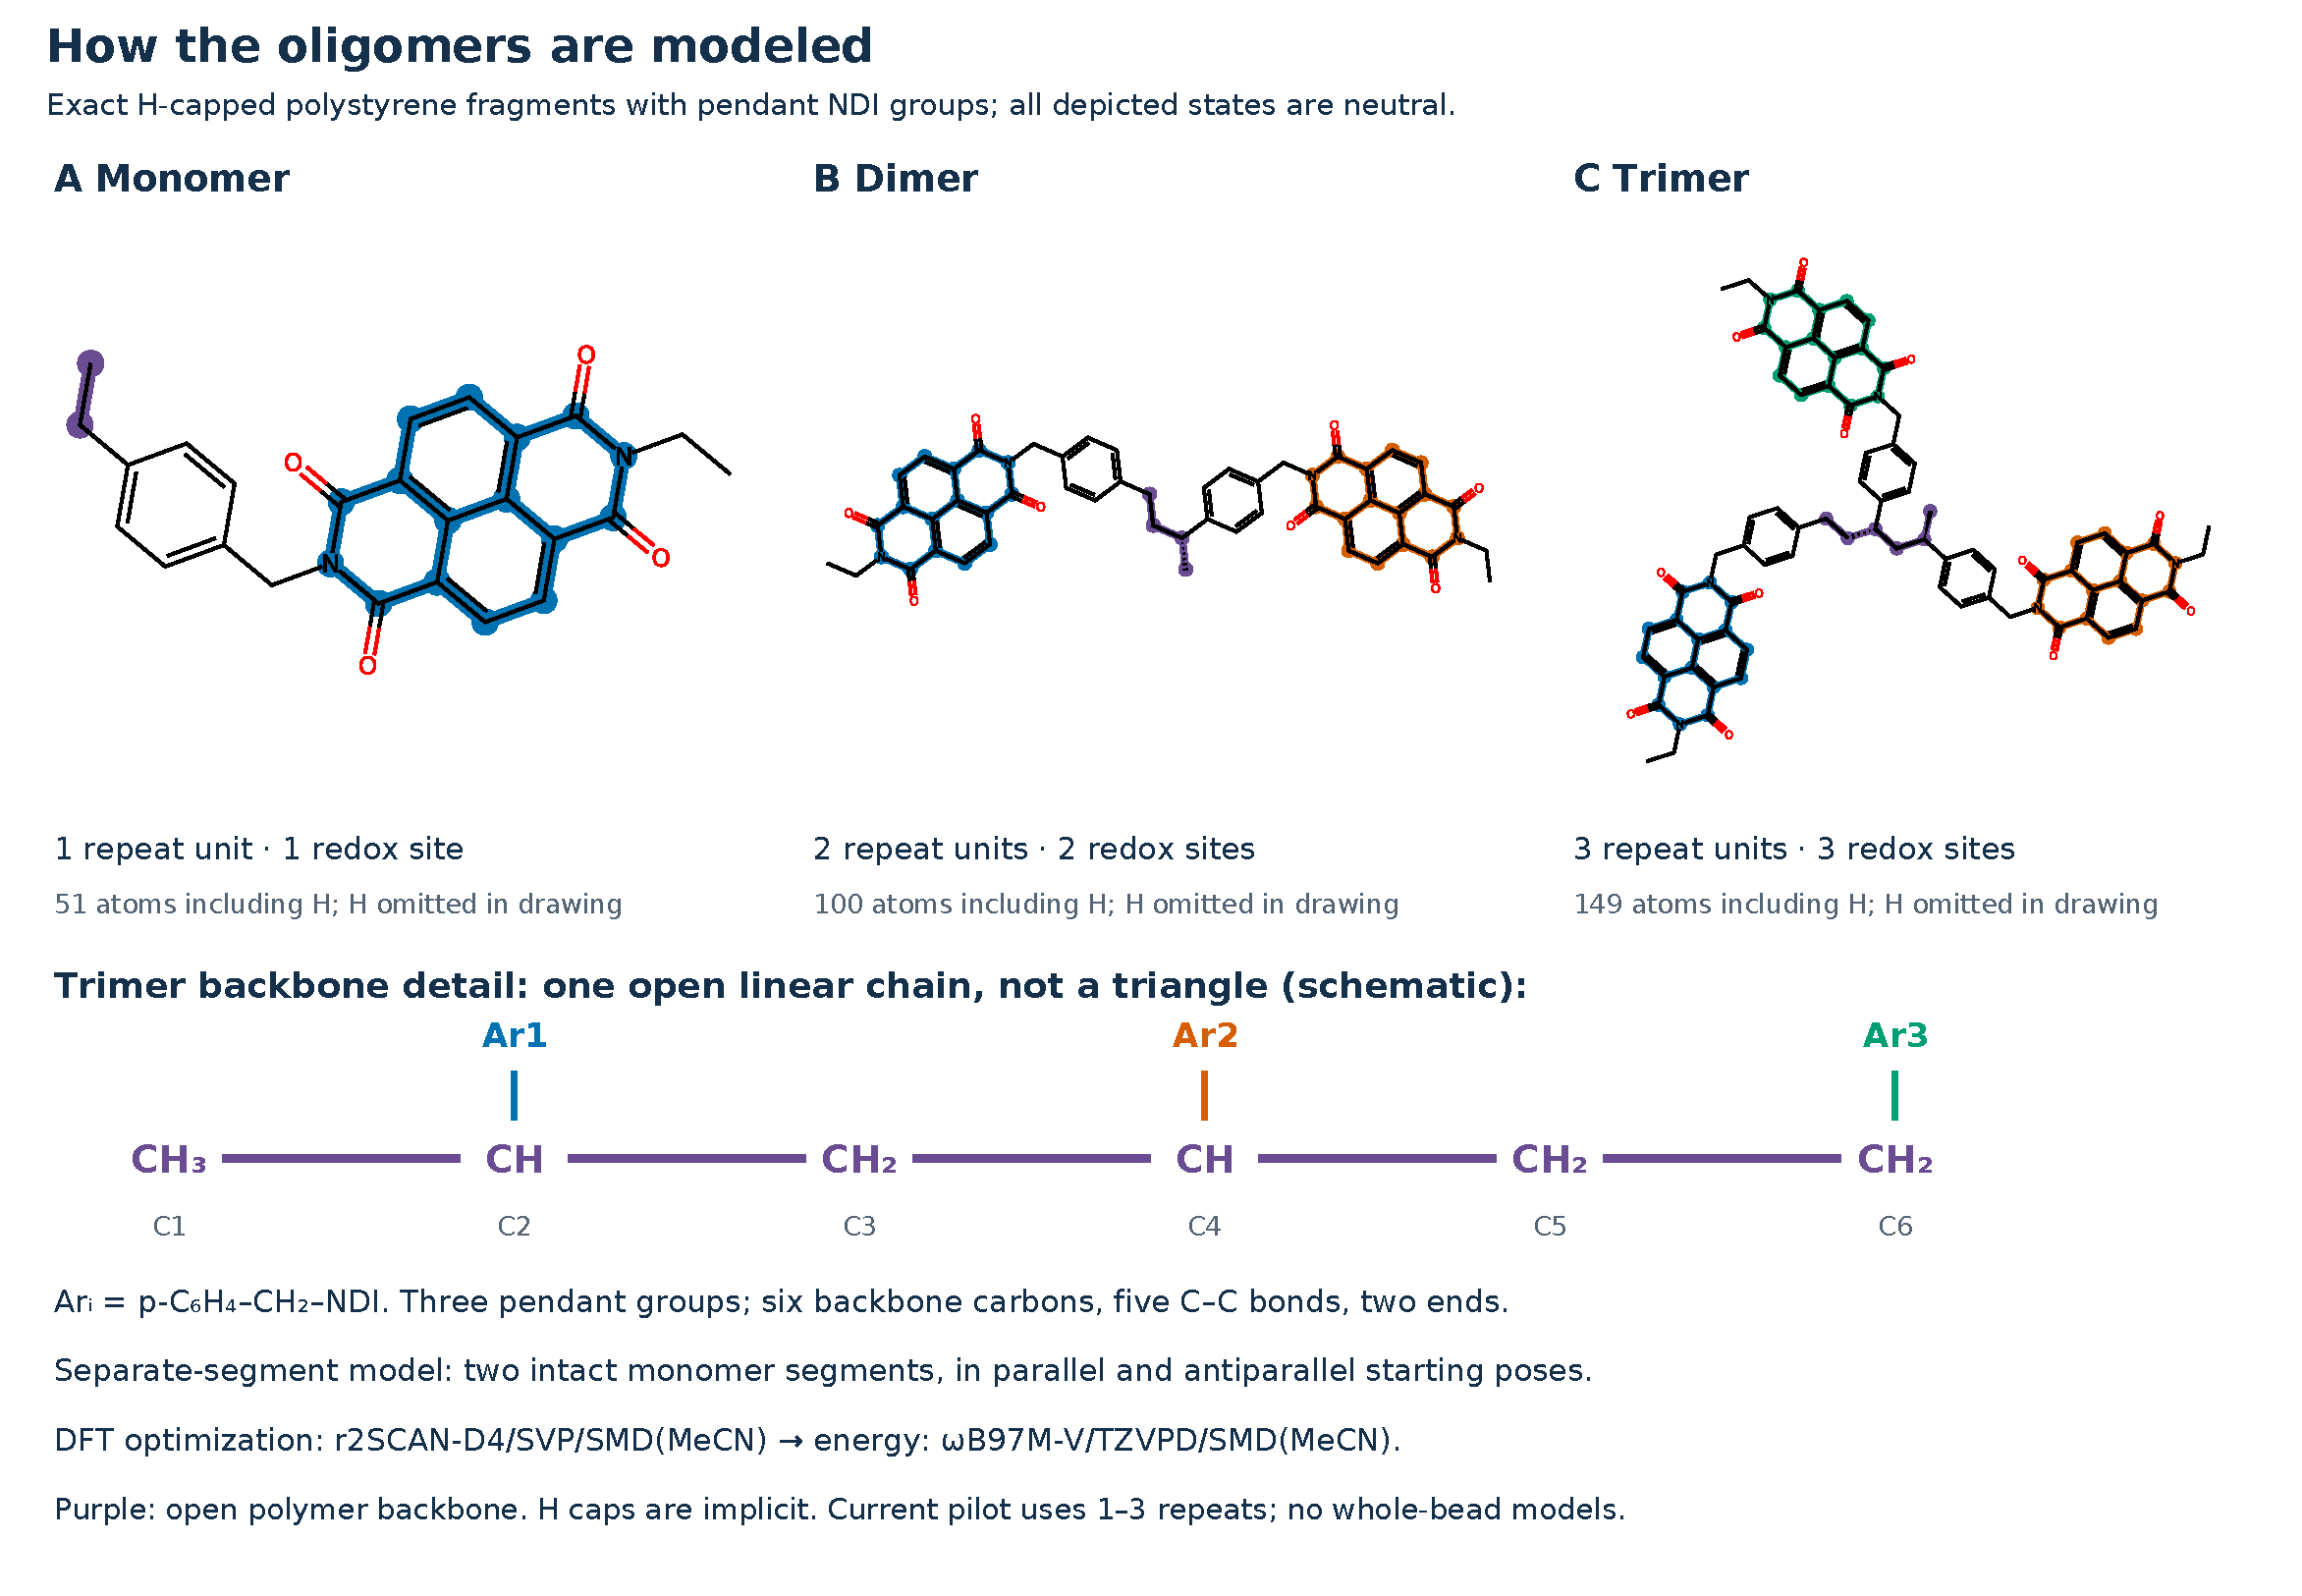
\includegraphics[width=\linewidth]{../results/figures/manuscript/2026-10-22_review_checked/construction.pdf}
\caption{Exact finite-polymer construction used in the interaction controls. The highlighted open backbone distinguishes covalent connectivity from spatial contacts among pendant groups. Monomer, dimer and trimer models are dense local scenarios and do not represent an experimentally measured sequence or graft-loading distribution.}
\label{fig:construction}
\end{figure}

\begin{figure}[htbp]\centering
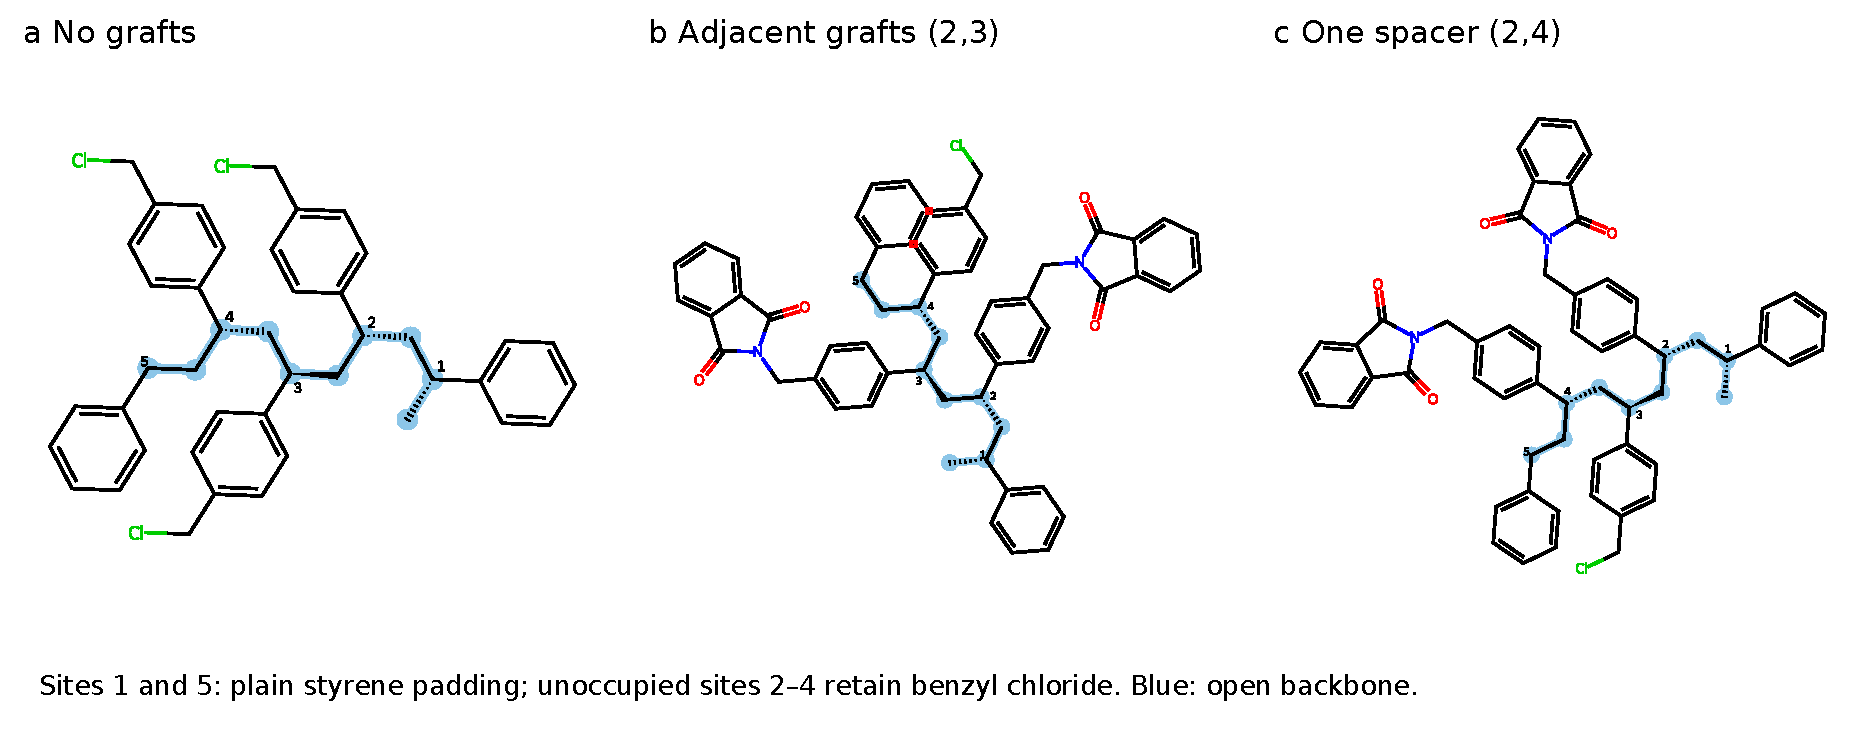
\includegraphics[width=\linewidth]{../results/figures/manuscript/2026-10-22_review_checked/spacing_construction.pdf}
\caption{Exact five-repeat phthalimide graphs used in the occupancy cycles. Blue highlights the open ten-carbon backbone. Sites 1 and 5 are plain styrene padding; unoccupied reactive sites retain benzyl chloride. Numbers label repeat positions, and stereobonds retain the declared configuration. These are connectivity drawings, not sampled spatial conformations. Single-occupancy reference graphs are included in the evidence.}
\label{fig:spacingconstruction}\end{figure}
For the six-graph spacing control, all twelve electronic conformers qualify. The selected electronic nonadditivities are $-10.98$ and $-14.50$ \kj\ for adjacent and one-spacer grafts, respectively. These refer to a matched empty-backbone minimum within the declared, limited sampling set. It demonstrates why a matched empty-backbone reference is necessary; it does not establish a universal distance trend.

All six selected-geometry native free energies now qualify, and both occupancy cycles close independently. Their largest Cartesian gradient components range from $1.01\times10^{-5}$ to $7.62\times10^{-5}$ hartree bohr$^{-1}$. The adjacent and one-spacer $\Delta\Delta G$ values are $-5.15$ and $-11.23$ \kj, respectively (Figure~\ref{fig:conditional}). Changing the rotor cutoff among 25, 50 and 100 cm$^{-1}$ gives ranges of $-5.15$ to $-4.66$ and $-12.14$ to $-11.23$ \kj. These ranges describe partition sensitivity; they are not statistical confidence intervals or conformational ensemble uncertainties.

For DBU and separated ions, grafting site $j$ onto an empty backbone gives $-110.87$ \kj\ at site 3 and $-103.41$ \kj\ at site 4. When site 2 is already grafted, these values become $-116.02$ and $-114.64$ \kj. The contact-pair alternatives are $-115.66$ to $-120.82$ \kj\ for site 3 and $-108.21$ to $-119.43$ \kj\ for site 4. Both attachment orders obey the same nonadditivity cycle. Thus a prior graft changes the conditional thermodynamics in this finite control. A more negative second-attachment free energy is not automatically a desirable materials property when weak unwanted neighboring-site interactions are the objective.

\begin{figure}[htbp]
\centering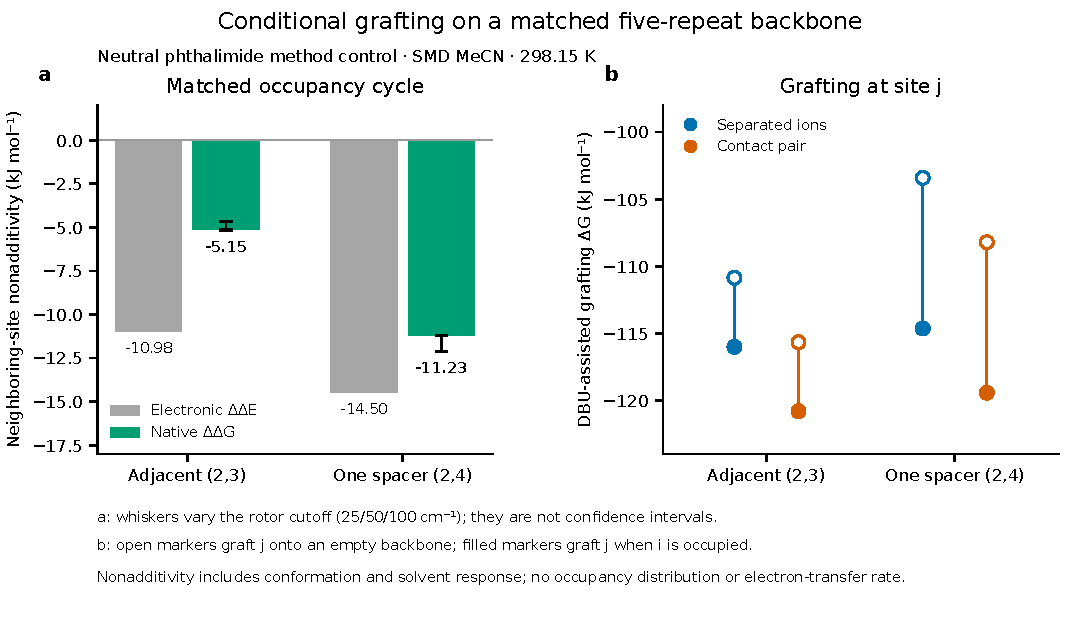
\includegraphics[width=\linewidth]{../results/figures/manuscript/2026-10-22_review_checked/conditional_grafting.pdf}
\caption{Conditional grafting in a matched five-repeat neutral phthalimide method control in MeCN at 298.15 K. Electronic and native free-energy nonadditivity are distinct. Whiskers vary only the rotor cutoff. Open and filled markers compare attachment at $j$ without and with a graft at $i=2$. All six selected geometries pass native QC, but the two conformers per graph do not establish an ensemble or a general spacing trend. Energies include backbone, conformational and solvent contributions.}
\label{fig:conditional}
\end{figure}
\pending{Resolve the final trimer slot and add representative redox-core and conformational sensitivity before making general polymer-design claims.}

The intact-segment decomposition is complete for three sampled pairs using six frozen-fragment single-point calculations (Figure~\ref{fig:decomposition}). Its partition separates interactions at the complex geometry from deformation relative to relaxed fragments. The interaction energies are $-55.25$, $-44.30$ and $-50.87$ \kj, with deformation terms $+0.56$, $+0.49$ and $+0.38$ \kj, respectively. Small deformation terms describe proximity to the selected isolated-reference geometries; they do not demonstrate equilibrated segment conformations. The extent of complex relaxation and reference selection requires a separate audit. The resulting quantities remain electronic, uncorrected for basis-set superposition error and inclusive of backbone and cap contributions. No electron-transfer rate follows from their magnitude.

\begin{figure}[htbp]
\centering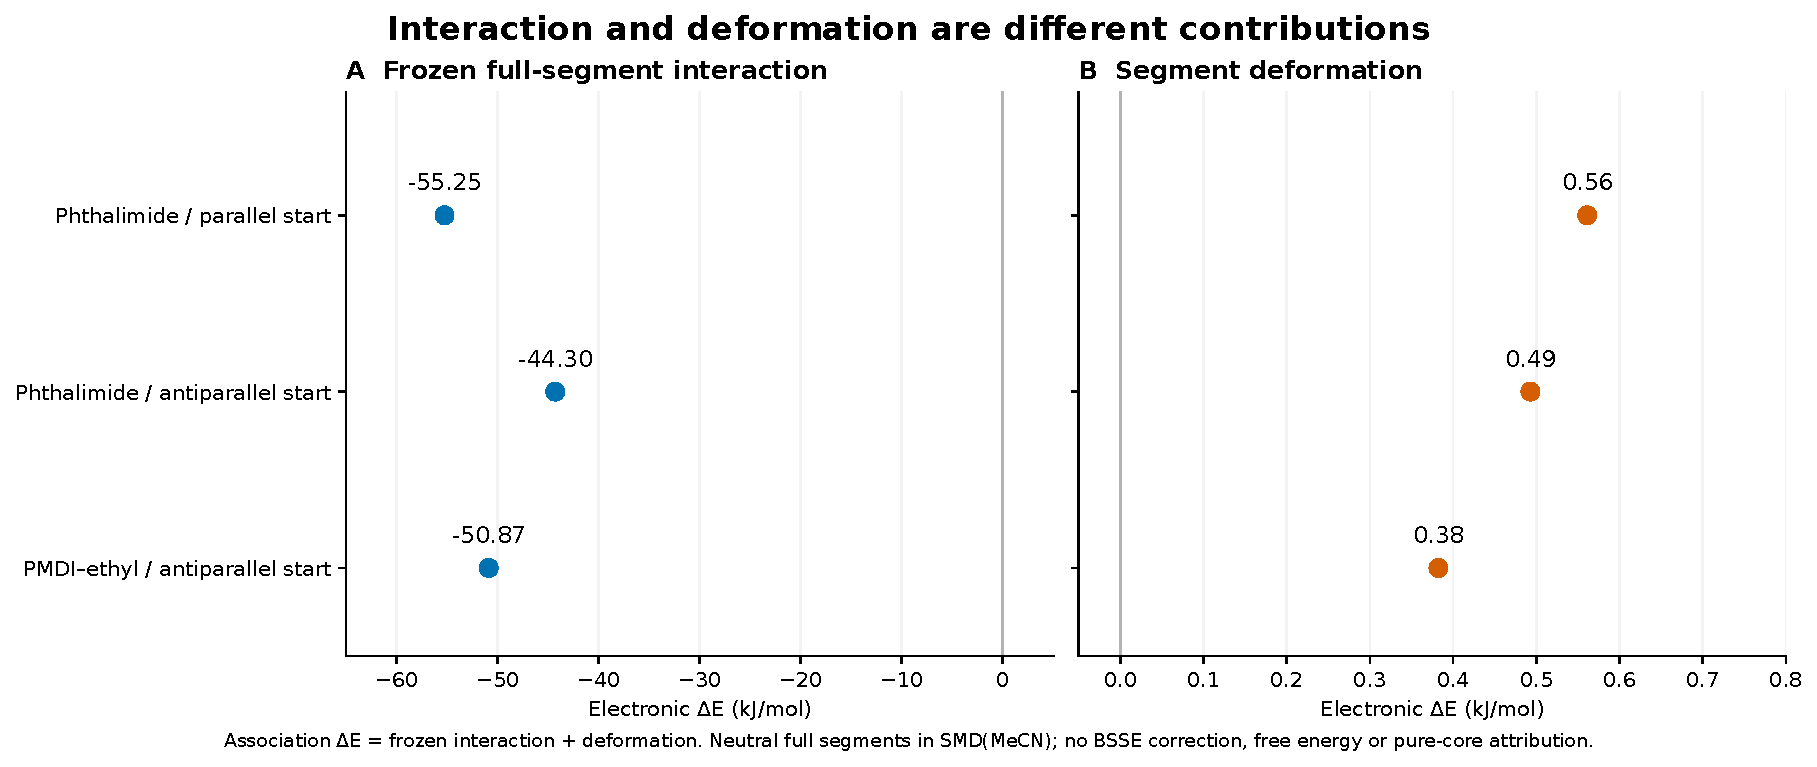
\includegraphics[width=\linewidth]{../results/figures/manuscript/2026-10-22_review_checked/decomposition.pdf}
\caption{Electronic interaction/deformation partition for three intact segment pairs. Frozen fragments retain the complex geometry without bond cutting or new caps. The partition closes the association-energy cycle but is not a pure pendant-core interaction, a counterpoise-corrected energy or an association free energy.}
\label{fig:decomposition}
\end{figure}

\section{Numerical implementation checks}
Diagnostics exposed distinct numerical issues. At a checkpoint of the open PMDI trimer, a legacy solvent cavitation--dispersion--solvent-structure (CDS) force component disagrees with total-energy finite differences by approximately $1.81\times10^{-4}$ hartree bohr$^{-1}$ at the tested coordinate on both integration grids. This discrepancy is not resolved by electronic-grid refinement. Conservative CDS energy derivatives reproduce the tested total-energy differences; their step consistency is checked before use in a continuation. Adaptive refinement of unresolved CDS derivative components recovers the open-trimer optimization. At the returned geometry, independent total-energy derivatives at two step sizes and two tested coordinates agree within $4.2$--$5.0\times10^{-7}$ hartree bohr$^{-1}$, below the unchanged $10^{-6}$ check threshold. This establishes an admitted stationary electronic geometry; no native-Hessian minimum or association free energy is inferred for that original oligomer case.

For the largest spacing Hessian, the original CDS finite-difference step produces a total asymmetry of $2.06\times10^{-6}$, exceeding the fixed $10^{-6}$ admission threshold. A separately qualified finer step reduces this to $2.05\times10^{-8}$. Additive reconstruction replays complete singlet and radical recomputations with maximum matrix differences of $1.33\times10^{-11}$ and $2.83\times10^{-9}$ atomic units, and thermal differences below $1.2\times10^{-8}$ eV. The recovered target then passes the ordinary native gates, with a lowest internal frequency of $+7.23$ cm$^{-1}$. These are execution-equivalence results, not a relaxation of physical QC or a high-level validation of grafting energetics.

\section{Execution and restart controls}
A synthetic control packs one million distinct tasks into one thousand chunks in 75.9 s with a measured preparation peak RSS of 67.2 MiB. Eight workers on two hosts execute the synthetic tasks over a 9.58 s span, excluding packing and startup. Independent arithmetic checks find zero discrepancies. This timing characterizes scheduling and storage, not chemical enumeration, conformer search or DFT throughput.

Separately, all 837 molecular descriptor outputs agree with serial definitions. In the shared-filesystem recovery experiment, 32 real design recipes deduplicate to 17 exact molecular tasks. A worker on one host exits abruptly after four checkpointed tasks; owner verification on that host precedes recovery. A second host completes the remaining thirteen tasks without repeating the four checked tasks. All resumed outputs match uninterrupted execution and a separate serial replay. This experiment tests descriptor-stage recovery. A distinct quantum interruption experiment is described below; neither establishes million-molecule quantum throughput.
A seeded randomized concurrency experiment executes the same 837 exact designs fifteen times, with three repeats per condition and eight tasks per chunk. All 12,555 molecular comparisons match the independent serial definition. Median launch-to-observed completion times are 4.436, 3.147, 2.680 and 2.497 s for one, two, four and eight CPU workers on one host; eight workers across two hosts require 2.585 s (Figure~\ref{fig:concurrency}). These times include node preflight, SSH, scorer initialization, execution and at most 0.1 s of observation polling; preparation is separate. All requested workers finish, but only seven of eight execute chunks in one single-host repeat. The diminishing returns of this small library do not determine an optimal concurrency for larger or more expensive stages.

A separate sparse Git checkout and newly installed Python 3.11 CPU environment reproduce the declared 32-recipe / 17-design example with system and user site packages disabled. The project loads from that checkout and scientific dependencies load from the new environment. Serial descriptor replay, exact-route holds and the regenerated conditional-grafting table all match; rendered RGB pixels of the figure are identical. This qualifies a small CPU reproduction using curated scientific data. It does not recompute the underlying quantum energies or qualify the complete CUDA environment.

\begin{figure}[htbp]
\centering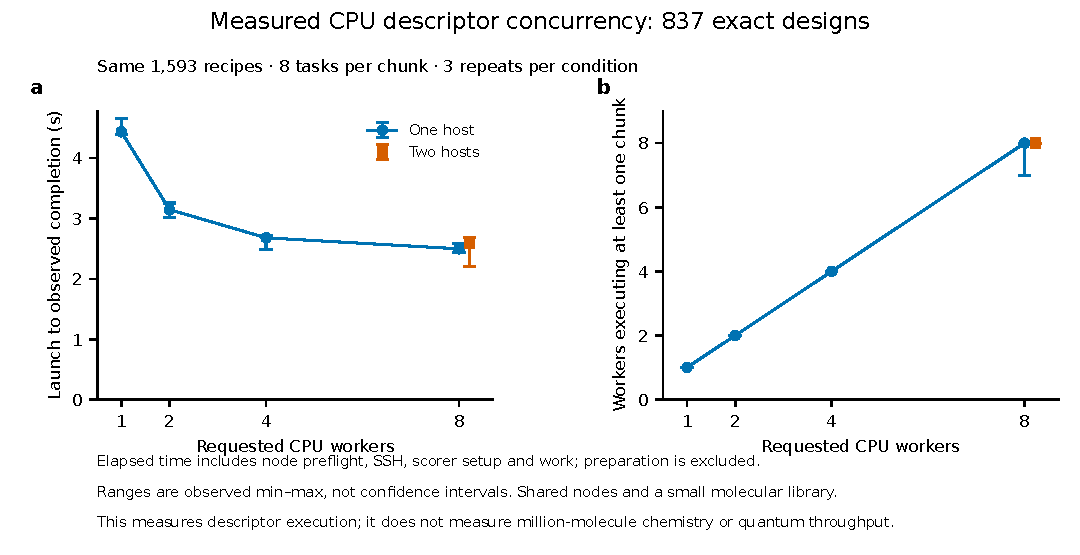
\includegraphics[width=\linewidth]{../results/figures/manuscript/2026-10-22_review_checked/cpu_concurrency.pdf}
\caption{Measured CPU descriptor concurrency for the same 837 exact designs. Three randomized repeats per condition retain every result. Ranges are observed minima and maxima, not confidence intervals. Launch, preflight and scorer overhead are included; preparation is separate. Requested workers and workers executing at least one chunk are distinct. This shared-node, small-library experiment does not measure million-molecule chemistry or quantum throughput.}
\label{fig:concurrency}
\end{figure}
\pending{Complete conformer-stage adapters, broader quantum recovery controls and accessible archival packaging. Keep stage-specific throughput separate from scientific accuracy.}


\subsection{Actual quantum interruption and recovery}
Two rigid controls, formaldehyde (singlet) and methyl radical (doublet), compare uninterrupted calculations with a fresh process resumed after an intentional exit following three durable gradient evaluations. The exit code is 87; process and start identity confirm termination before resubmission. The saved geometry is unqualified until optimization, active electronic energy, DFT Hessian, projected partition, topology and spin checks pass normally. Acceptance tolerances were $10^{-5}$ eV for electronic energy, $10^{-4}$ eV for free energy, $10^{-3}$ \AA\ aligned RMSD and 0.5 cm$^{-1}$ for internal frequencies. Singlet differences are $4.03\times10^{-6}$ eV, $1.26\times10^{-5}$ eV, $6.87\times10^{-6}$ \AA\ and 0.0685 cm$^{-1}$; doublet differences are $4.00\times10^{-6}$ eV, $1.11\times10^{-6}$ eV, $3.45\times10^{-5}$ \AA\ and 0.0264 cm$^{-1}$. Four final partitions were independently reconstructed. This verifies restart equivalence for these two controls, not flexible-polymer sampling or chemical accuracy.
\Needspace{19\baselineskip}
\section{Evidence terminology}
\begin{table}[H]\centering\small
\caption{Terms used in evidence files and their interpretation.}
\begin{tabular}{p{.24\linewidth}p{.67\linewidth}}\toprule
Term & Meaning\\\midrule
Exact design & A specified precursor/product graph and mapped attachment bond; generating recipes can deduplicate to the same design.\\
Checked or qualified & The checks required for the named field passed; this is not experimental validation.\\
Native free energy & Active electronic energy plus the projected geometry-level DFT nuclear partition and declared spin partition.\\
Frozen snapshot & An immutable, hash-verified copy of specified evidence; newer live results require a new snapshot.\\
Proceed / hold / exclude & Route decisions within the stated evidence scope; hold means required exact-route evidence is incomplete.\\
Endpoint & One sourced redox-potential comparison, with exact molecular identity, state pair and reference convention.\\
Pose & One conformational starting geometry; the final optimized contact class is checked separately.\\
\bottomrule\end{tabular}\end{table}
\bibliographystyle{unsrtnat}\bibliography{references}
\end{document}
